\documentclass{standalone}
\usepackage{tikz}

\begin{document}
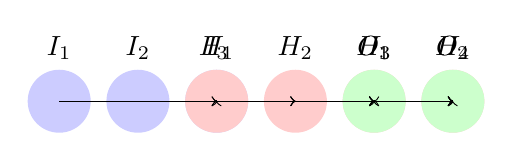
\begin{tikzpicture}[x=1cm,y=1cm]
    % Define layers' positions
    \def\layersep{2} % separation between layers
    
    % Draw input layer (3 neurons)
    \foreach \x [count=\i] in {1,2,...,3} {
        \node[circle,fill=blue!20,minimum size=0.8cm] at (\x,0) {};
        \node[above] at (\x,0.4) {$I_{\i}$}; % label each neuron
    }
    
    % Draw hidden layer (4 neurons)
    \foreach \x [count=\i] in {1,2,...,4} {
        \node[circle,fill=red!20,minimum size=0.8cm] at (\x+\layersep,0) {};
        \node[above] at (\x+\layersep,0.4) {$H_{\i}$}; % label each neuron
    }
    
    % Draw output layer (2 neurons)
    \foreach \x [count=\i] in {1,2} {
        \node[circle,fill=green!20,minimum size=0.8cm] at (\x+2*\layersep,0) {};
        \node[above] at (\x+2*\layersep,0.4) {$O_{\i}$}; % label each neuron
    }
    
    % Draw connections between layers using foreach loop
    \foreach \x in {1,2,...,3} {
        \foreach \y in {1,2,...,4} {
            \draw[->] (\x,0) -- (\y+\layersep,0);
        }
    }
    \foreach \x in {1,2,...,4} {
        \foreach \y in {1,2} {
            \draw[->] (\x+\layersep,0) -- (\y+2*\layersep,0);
        }
    }
\end{tikzpicture}
\end{document}